\documentclass{article} % For LaTeX2e
\usepackage{iclr2025_conference,times}

\input{math_commands.tex}

\usepackage{hyperref}
\usepackage{url}
\usepackage{graphicx}
\usepackage{booktabs}
\usepackage{multirow}
\usepackage{amsmath,amssymb,amsthm}

\newtheorem{theorem}{Theorem}
\newtheorem{proposition}{Proposition}
\newtheorem{definition}{Definition}
\newtheorem{corollary}{Corollary}
\newtheorem{lemma}{Lemma}
\newtheorem{remark}{Remark}
\newtheorem{example}{Example}

\newcommand{\dftext}{distortion-free}
\newcommand{\Ecal}{\mathcal{E}}

\title{Distortion-Free Until You Select:\\
Watermarking under Best-of-$N$ Inference}

% Anonymized for submission
\author{Anonymous authors\\
\texttt{anon@example.com}}

\newcommand{\fix}{\marginpar{FIX}}
\newcommand{\new}{\marginpar{NEW}}

\iclrfinalcopy % TODO: comment out for anonymous submission
\begin{document}

\maketitle

\begin{abstract}
Distortion-free watermarks guarantee that a \emph{single} generation is distributed
identically to unwatermarked text. Modern deployments, however, rarely release a single
sample: inference-time selection --- Best-of-$N$ (BoN) sampling with a reward model,
reranking, self-consistency --- chooses among $N$ candidates. We show that the standard
guarantee is \emph{not closed under selection}: with the deployed family of
context-hashed, deterministic-key schemes (Gumbel/Aaronson-style), the $N$ candidates
for a prompt are generated from the same pseudorandom stream and collapse to $N$
identical copies, so BoN forfeits its entire alignment gain; the practical workaround
--- softening the sampler --- restores diversity but sacrifices the distortion-free
property that motivated the scheme. We formalize \emph{$N$-selection-closed}
distortion-freeness and prove that joint preservation is \emph{necessary and
sufficient} for closure under every selection operator --- marginal
preservation alone controls nothing --- and give a
\emph{general lifting}, not another watermarking algorithm: the jointly-coupled
transform $\mathrm{JC}_N$ compiles \emph{any} keyed watermarking scheme into a
selection-closed one by domain-separated per-candidate subkeys under a single
master key, and lifts the scheme's own detector by a union wrapper whose cost is
a once-per-sequence $\sqrt{2\ln N}$ threshold shift. The guarantees are
scheme-agnostic and selector-agnostic. Instantiated on the deployed
Gumbel/Aaronson scheme, the lifted system restores the full BoN reward gain of
unwatermarked sampling (reward $0.0861$ vs.\ ceiling $0.0848$ on
LLaMA-3.1-8B-Instruct) while remaining strictly distortion-free, retains
detection at $\approx0.3$ z-score cost, and Pareto-dominates the deployed
softened workaround on reward, detection, and distributional correctness
simultaneously.
\end{abstract}

\section{Introduction}
% Hook: inference-time compute is the norm; watermarks are certified sample-wise.
Watermarking schemes for large language models are certified by a \emph{single-sample}
guarantee: averaged over the secret key, one generation is distributed exactly as
unwatermarked text \citep{aaronson2023, kuditipudi2023robust, zhao2024permute}.
Deployed systems, however, increasingly ship \emph{selection} on top of generation:
Best-of-$N$ sampling against a reward model recovers the alignment that watermarking
degrades \citep{verma2025watermarking}, rerankers and verifiers choose among drafts,
and self-consistency votes over samples. This paper asks a simple question:
\begin{center}
\emph{Does distortion-freeness survive inference-time selection?}
\end{center}
We show that it does not --- quantitatively, catastrophically, and for the exact
scheme family that is deployed today --- and that a one-line fix closes the gap.

\textbf{The collapse.} In context-hashed deterministic schemes (Gumbel/Aaronson-style,
KGW derivatives, SynthID-Text), the per-step noise is a pseudorandom function of the
key and the local context. All $N$ BoN candidates for a prompt start from the same
context, so they read the same noise and make the same argmax choice --- and identical
prefixes are a fixed point of the dynamics, so the candidates remain identical
forever: generation is a deterministic function of (key, prompt), and no step ever
creates a first divergence. On LLaMA-3.1-8B-Instruct we observe exactly $1/16$
unique candidates per prompt --- Figure~\ref{fig:transcript} shows a verbatim
instance. Selection then has nothing to select from: every
selection head returns the single-sample reward ($0.0693$), forfeiting the entire
BoN gain (unwatermarked BoN reaches $0.0848$ at $N{=}16$). More generally, marginal
correctness with joint correlation suffices to bias \emph{any} selector, and the bias
\emph{grows} with $N$ (Figure~\ref{fig:toy}; in the comonotone worst case ---
realized by the deployed scheme --- the shift approaches TV $=\tfrac12$,
Example~\ref{ex:comonotone}). The de facto workaround --- softening the sampler with
fresh randomness \citep{verma2025watermarking} --- restores diversity but breaks the
strict distortion-free property it was meant to protect, and we show it is in fact
strictly dominated by our construction.

\textbf{Folklore vs.\ what is new.} That fixed-seed deterministic decoding
returns identical outputs is known as an operational nuisance
\citep{verma2025watermarking}. What has been missing is the consequence for the
\emph{certified guarantee}: distortion-freeness is certified per sample but
deployed under selection, and no prior analysis addressed (i) what selection
does to the guarantee (it forfeits the entire BoN gain; in the worst case ---
realized by the deployed scheme --- the output shift approaches
$\mathrm{TV}=\tfrac12$), (ii) whether the accepted workaround is sound
(softening is strictly dominated and remains correlated), (iii) what the right
property is (joint preservation, exactly characterized below), and (iv) what
restoring it costs at detection ($\sqrt{2\ln N}$, once per sequence, and
order-optimal). The phenomenon is folklore; the broken guarantee, its
quantification, and the closed-loop fix are not.

\textbf{Formalization.} We define \emph{$N$-selection-closed} distortion-freeness:
the joint distribution of the $N$ candidates (and hence of the output of \emph{any}
selection operator applied to them) matches that of $N$ i.i.d.\ unwatermarked samples.
Single-sample (marginal) distortion-freeness does not imply it; joint
preservation is exactly the right condition --- necessary and sufficient
(Theorem~\ref{thm:closure}). The property sits strictly between the
deployed weak guarantee and cryptographic undetectability
\citep{christ2023undetectable}, which implies it computationally but has no deployed
instantiation (Proposition~\ref{prop:hierarchy}).

\textbf{Framework.} We emphasize what this paper is \emph{not}: it proposes no
new watermarking algorithm. Instead we give a scheme-agnostic \emph{lifting},
the jointly-coupled transform $\mathrm{JC}_N$: given any keyed sampler $W$
whose per-step randomness is a pseudorandom function of its key, candidate $i$
runs $W$ unmodified under
$\mathrm{SubKey}_i=\mathrm{PRF}(\mathrm{MasterKey},\,i)$. One master key is
kept; the $N$ candidates become (computationally) i.i.d.\ copies of $W$'s
single-sample law, so whatever marginal guarantee $W$ has is inherited
\emph{jointly} --- in particular, marginally distortion-free $W$ becomes
$N$-selection-closed (Theorem~\ref{thm:lifting}), for every selection operator.
Detection lifts the same way: the \emph{union wrapper} runs $W$'s own detector
under each subkey (only $N$, or an upper bound, need be known --- not the
selected index), paying a once-per-sequence threshold penalty of
$\sqrt{2\ln N}$ --- empirically $0.3$ z-score at $N{=}16$ against a signal of
$z\approx7.7$ --- and recovering the winning candidate's index as a free audit
log. Figure~\ref{fig:detectors} verifies that the union detector matches the
correct-subkey oracle at every $N$ and entropy level.

\textbf{Results.} On LLaMA-3.1-8B-Instruct with HH-RLHF prompts and an ArmoRM reward:
(i) strict shared-key BoN returns identical candidates and zero BoN gain;
(ii) subkeys restore $16/16$ unique candidates and full BoN reward
($0.0861 \ge$ unwatermarked ceiling $0.0848$), with single-sample reward matching
the unwatermarked model ($0.0698$ vs.\ $0.0703$; strict distortion-freeness);
(iii) union detection retains $z=7.71$ vs.\ $8.00$ for the shared key;
(iv) the softened workaround is dominated on all three axes simultaneously
(reward $0.0861$ vs.\ $0.0852$; post-BoN detection $z$ $6.50$ vs.\ $5.62$; strict
vs.\ broken distortion-freeness).

\textbf{Contributions.}
\begin{enumerate}
  \item We identify and quantify the failure of single-sample distortion-freeness
        under inference-time selection, on the deployed scheme family
        (\S\ref{sec:collapse}).
  \item We formalize $N$-selection-closedness, characterize it exactly (joint
        preservation is necessary and sufficient for closure under every
        selector), quantify the mechanism (candidate correlation $\rho$
        attenuates the selection gain by $\sqrt{1-\rho}$,
        Lemma~\ref{lem:attenuation}), and place the notion in a hierarchy
        between marginal distortion-freeness and undetectability
        (\S\ref{sec:theory}).
  \item We give the general jointly-coupled transform $\mathrm{JC}_N$ --- a
        compiler that lifts \emph{any} keyed watermarking scheme to a
        selection-closed one under a single master key
        (Theorem~\ref{thm:lifting}) --- together with the lifted union
        detection and its once-per-sequence $\sqrt{2\ln N}$ cost analysis
        (\S\ref{sec:method}).
  \item Instantiating the framework on the deployed Gumbel/Aaronson scheme, a
        real aligned model shows full recovery of the BoN gain at strict
        distortion-freeness, and strict dominance over the deployed softened
        workaround (\S\ref{sec:experiments}).
\end{enumerate}

\section{Related Work}\label{sec:related}
\textbf{Distortion-free watermarking.}
Gumbel/exponential schemes \citep{aaronson2023}, inverse-transform and robust
variants \citep{kuditipudi2023robust}, permute-and-flip \citep{zhao2024permute},
and semantic-level schemes \citep{pmark2025} certify a single-sample
(or key-averaged) distributional guarantee. SynthID-Text \citep{dathathri2024scalable}
deploys the context-hash family at scale with repeated-context masking, which
addresses intra-sequence reuse, not cross-candidate correlation.

\textbf{Key reuse and collisions.}
\citet{keycollision2024} prove that key collisions across generations induce
correlations and break distortion-freeness of the \emph{generated} text distribution.
Our setting is the extreme collision --- $N$ candidates for one prompt collide at
every step --- and our observation is one level higher: a \emph{selection operator}
converts joint correlation into first-order bias of the \emph{deployed output}.
The random-offset construction of \citet{kuditipudi2023robust} decorrelates
candidates approximately, at the cost of alignment-based (edit-distance) detection;
our fix keeps the strong context-hash detectors.

\textbf{Selection and watermarks.}
Alignment Resampling \citep{verma2025watermarking} uses reward-based BoN on
watermarked models and explicitly sacrifices strict distortion-freeness for
diversity; we show this workaround is dominated. WaterMax
\citep{giboulot2024watermax} and WaterSearch \citep{watersearch2025} use
multi-draft selection \emph{for} the watermark (choosing drafts by watermark score),
the dual of our setting; WaterSearch also employs per-candidate seeds as a mechanism,
without a selection-closure analysis. Multi-bit watermarking decodes a message by
running detection under every message key and taking the best p-value
\citep{fernandez2023three}; our union wrapper inherits this standard practice.
Unlike this line of work, we propose no new watermarking scheme: our object of
study is the \emph{transform} that any keyed scheme composes with, and its
guarantees are proved once for all schemes and selectors.

\textbf{Undetectability.}
\citet{christ2023undetectable} construct watermarks that are computationally
undetectable under adaptive multi-query access, which implies selection-closure
computationally; the construction is not practical for deployment. Our notion is the
minimal targeted property, and our fix upgrades the deployed family in place
(Proposition~\ref{prop:hierarchy}).

\section{The Selection Collapse}\label{sec:collapse}

\begin{figure}[t]
\centering
\fbox{\begin{minipage}{0.95\linewidth}\small
\textbf{Prompt} (HH-RLHF): \emph{``I've been seeing a lot of slugs outside
recently, even crawling up trees. Should I do something about them, or just
let them be?''}\\[3pt]
\textbf{Strict shared key} --- all $16$ ``Best-of-16'' candidates, verbatim:\\
{\ttfamily That's an interesting sight! Slugs can be quite fascinating
creatures. As for whether you should do something about them, it depends on a
few factors.\,\ldots}\hfill$\times16$\\[3pt]
\textbf{Jointly-coupled lift (per-candidate subkeys)} --- first three of $16$
distinct candidates:\\
{\ttfamily That's an interesting observation! Slugs can indeed be quite\,\ldots}\\
{\ttfamily That's an interesting observation! Slugs can be quite resilient\,\ldots}\\
{\ttfamily That's an interesting observation! Slugs can be quite adaptable\,\ldots}
\end{minipage}}
\caption{The collapse, verbatim (LLaMA-3.1-8B-Instruct, Gumbel watermark,
$N{=}16$, same prompt). Under the strict shared key the Best-of-$16$ pool is
sixteen byte-identical copies of one sample --- selection has nothing to
select --- while the lift returns sixteen genuinely distinct candidates.}
\label{fig:transcript}
\end{figure}

% Mechanism: determinism + identical initial condition -> identical trajectories.
\subsection{Setup}
Let $\pi$ denote the language model, $x$ a prompt, and consider $N$ candidate
generations $Y_1,\dots,Y_N$ produced by a watermarked decoder with key $k$.
A \emph{selection operator} $S$ (e.g., $\arg\max$ of a reward model $r$) returns
$Y_{S}$. In context-hash schemes, the per-step noise at position $t$ is
$g_t = \mathrm{PRF}(k, \mathrm{ctx}_t)$ where $\mathrm{ctx}_t$ is the local
$h$-gram context, and the token is chosen by a deterministic rule (argmax) given
logits and noise.

\subsection{A thirty-second failure}\label{sec:coin}
Let each candidate be a fair coin flip and let the selector prefer heads. With
i.i.d.\ candidates, Best-of-$N$ returns heads with probability $1-2^{-N}$. Now
couple the candidates into $N$ copies of a \emph{single} flip: every copy is
still a perfectly fair coin --- the certified, marginal guarantee is intact ---
yet the selector returns heads with probability $\tfrac12$. The deployed
output laws differ by $\mathrm{TV}=\tfrac12-2^{-N}\to\tfrac12$: marginal
correctness survives, the deployed guarantee does not, and the gap grows with
the very compute ($N$) that selection adds. The strict shared key realizes
exactly this coupling (Figure~\ref{fig:transcript});
Example~\ref{ex:comonotone} gives the general statement.

\subsection{Identical candidates: an induction}
All candidates share the prompt, hence the initial context, hence the initial noise
and the initial token; by induction every subsequent context, noise, and token
coincide. Identical prefixes are a fixed point of the dynamics and the process
starts in it: generation is a deterministic function of $(k,x)$, so the $N$
candidates are $N$ copies. There is no source of a first divergence.
Empirically (\S\ref{sec:experiments}): $1.0/16$ unique candidates per prompt under
the strict shared key; the softened variant diverges stochastically but retains a
$2.2\times$ longer shared prefix than unwatermarked sampling
(Appendix~\ref{app:exp}).

\subsection{A minimal model of selection bias}\label{sec:toy}
Marginal correctness with joint correlation suffices to bias any selector.
We construct candidates with exact marginals and tunable correlation $\rho$
(Gaussian copula), select by noisy reward, and measure the total-variation
distance between the selected-output distribution and unwatermarked BoN
(Figure~\ref{fig:toy}). At $N{=}1$ the shift is zero for all $\rho$ (the classical
guarantee); for $N>1$ it grows with $N$ (TV $0.16\to0.55$ at $\rho{=}0.9$),
the candidate set's effective diversity collapses ($4.9\to2.5$ distinct answers
of $5$ at $N{=}16$), and the selected reward drops accordingly. Independent
candidates ($\rho{=}0$, our fix) keep the curve at zero.
The mechanism admits a closed form:

\begin{lemma}[Correlation attenuates the selection gain]\label{lem:attenuation}
Let candidate rewards be exchangeable Gaussian with mean $\mu$, variance
$\sigma^2$ and pairwise correlation $\rho\in[0,1]$, and let
$m_N=\mathbb E[\max_{i\le N}Z_i]$ for i.i.d.\ standard normals
($m_N\sim\sqrt{2\ln N}$). Then the expected reward of hard-BoN is
$\mu+\sigma\sqrt{1-\rho}\,m_N$: the independent system's selection gain is
attenuated by exactly $\sqrt{1-\rho}$, so the deployed output trails
independent BoN by $(1-\sqrt{1-\rho}\,)\,\sigma\,m_N$ --- increasing in both
$\rho$ and $N$, and equal to the entire gain at $\rho=1$ (the shared-key
collapse). Proof in Appendix~\ref{app:proofs}.
\end{lemma}

\begin{figure}[t]
\begin{center}
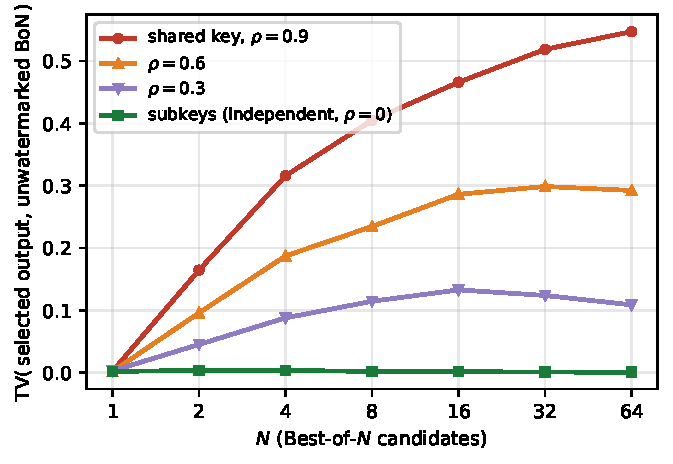
\includegraphics[width=0.62\linewidth]{figures/toy_select_shift.pdf}
\end{center}
\caption{Marginal preservation is not selection-closed. Each candidate's marginal is
exact (at $N{=}1$ the shift is $\approx 0$ for every $\rho$), yet shared-key
correlation ($\rho>0$) biases the selected output increasingly with $N$
(TV $0.16\!\to\!0.55$ at $\rho{=}0.9$); per-candidate subkeys ($\rho=0$) keep the
shift at zero. The shared-key deterministic scheme is the $\rho\to1$
(comonotone) extreme; Example~\ref{ex:comonotone} computes it in closed form.}
\label{fig:toy}
\end{figure}

\section{$N$-Selection-Closed Distortion-Freeness}\label{sec:theory}

\begin{definition}[$N$-selection-closed]\label{def:closure}
A watermarked sampler is \emph{exactly $N$-selection-closed} \dftext{} if, for
every prompt $x$, the joint law of its $N$ candidates equals
$Q_x^{\otimes N}$, the law of $N$ i.i.d.\ unwatermarked samples. It is
\emph{computationally} $N$-selection-closed if the two joint laws are
computationally indistinguishable. Statements below are for the exact notion;
each transfers verbatim to the computational one by composing the
distinguisher with the (efficient) selector.
\end{definition}

\textbf{Standing assumptions.} Selection operators observe the candidates and
auxiliary randomness independent of the watermark key; base samplers depend on
their key only through the keyed noise stream; the verifier knows $N$ or an
upper bound.

\begin{theorem}[Characterization of selection-closure]\label{thm:closure}
The following are equivalent:
(i) the joint law of the candidates equals $Q_x^{\otimes N}$ for every prompt;
(ii) for \emph{every} (possibly randomized) selection operator $S$ satisfying
the standing assumptions, the law of the selected output $Y_S$ equals that of
$S$ applied to unwatermarked i.i.d.\ candidates.
Moreover, marginal preservation alone does not imply (ii) for any $N\ge2$.
\end{theorem}
\begin{proof}[Proof sketch]
(i)$\Rightarrow$(ii): $Y_S$ is a measurable functional of the candidate tuple
and independent auxiliary randomness; equal joint laws have equal pushforwards.
(ii)$\Rightarrow$(i): probe selectors of the form ``pick $i$ if the other
coordinates fall in prescribed sets, else pick $j$'' identify every
finite-dimensional joint by induction on its order (Appendix~\ref{app:proofs}).
The final claim is witnessed by \S\ref{sec:toy}: exact marginals, correlated
joints, biased selection.
\end{proof}

\begin{proposition}[Hierarchy]\label{prop:hierarchy}
As classes of watermarked samplers,
\[
\{\text{undetectable}\}\;\subsetneq\;
\{\text{$N$-selection-closed}\}\;\subsetneq\;
\{\text{marginally \dftext}\}:
\]
(i) closure implies marginal \dftext{}ness (take the constant selector);
(ii) the converse fails --- the deployed context-hash family is marginally
\dftext{} yet not even $2$-selection-closed;
(iii) undetectability under adaptive queries \citep{christ2023undetectable}
implies $N$-selection-closedness computationally for every polynomial $N$;
(iv) the converse fails --- the lifted family is $N$-selection-closed yet
key-free distinguishable from response-collision statistics. Proofs in
Appendix~\ref{app:proofs}.
\end{proposition}

\section{The Jointly-Coupled Watermarking Framework}\label{sec:method}
This section is deliberately scheme-agnostic: we define a transform on
\emph{arbitrary} keyed watermarking schemes and prove its guarantees once, for
all schemes and all selectors. No new watermarking algorithm is introduced;
existing schemes are lifted unmodified.

\subsection{The $\mathrm{JC}_N$ transform}
A \emph{keyed sampler} $W$ is any watermarked decoder whose per-step
randomness is a deterministic (pseudorandom) function of a key $k$ and the
generation state, and whose key-dependence is \emph{only} through this noise
stream --- e.g., context-hash Gumbel/Aaronson, exponential/inverse-transform
sampling, tournament sampling, or biased-logit schemes with keyed sampling.
The \emph{jointly-coupled lift} $\mathrm{JC}_N(W)$ generates candidate
$i\in[N]$ by running $W$ \emph{unmodified} under the domain-separated subkey
$\mathrm{SubKey}_i=\mathrm{PRF}(\mathrm{MasterKey},\,i)$; in implementations
this is one line --- mix the candidate index into the seed-derivation chain.
One master key is stored; the derivation is free.

\begin{theorem}[Lifting]\label{thm:lifting}
Let $W$ be a keyed sampler with single-sample (key-averaged) output law
$\mu_W$.
(a) \emph{Ideal tier:} if the $N$ candidates are driven by truly independent
random streams, their joint law \emph{equals} $\mu_W^{\otimes N}$ --- total
variation exactly zero --- for any base scheme $W$, distortion-free or not.
(b) \emph{Real tier:} with streams derived from one master key by a PRF
($\mathrm{JC}_N$), the joint is computationally indistinguishable from
$\mu_W^{\otimes N}$: every polynomial-time observer --- any efficient selector
composed with any efficient downstream test --- has advantage at most the PRF
distinguishing advantage $\varepsilon$.
(c) If $W$ is marginally distortion-free ($\mu_W=Q$), then $\mathrm{JC}_N(W)$
is $N$-selection-closed (exactly in the ideal tier, up to $\varepsilon$ in the
real tier), and by Theorem~\ref{thm:closure} the released output under
\emph{any} selection operator is distributed as unwatermarked Best-of-$N$.
(d) Any detector for $W$ lifts to a detector for $\mathrm{JC}_N(W)$ (the union
wrapper of \S\ref{sec:detection}) with a once-per-sequence multiplicity cost.
\end{theorem}

\begin{proof}[Proof sketch]
(a) With independent streams the candidates are independent runs of $W$ by
construction. (b) A distinguisher against the candidate tuple composed with
the stream-generation map is a distinguisher against the PRF at $N$ distinct
inputs. (c) i.i.d.\ with marginal $Q$ is Definition~\ref{def:closure};
closure then follows from Theorem~\ref{thm:closure}. (d) is
Proposition~\ref{prop:union}. Full proof in Appendix~\ref{app:proofs}.
\qedhere
\end{proof}

\begin{remark}[$\varepsilon$ is the price of detectability]\label{rem:price}
Truly independent streams achieve exact closure but destroy the watermark:
with no key there is nothing to detect. The PRF is precisely what buys the
verifier reproducibility, and its $\varepsilon$ is the entire gap between the
tiers. Exact distortion-freeness and detectability are jointly unattainable;
$\mathrm{JC}_N$ attains both computationally.
\end{remark}

Parts (a)--(b) are worth emphasizing: even for schemes that are \emph{not}
distortion-free (e.g., biased-logit families with keyed sampling), the lift
restores candidate i.i.d.-ness, so selection behaves as ordinary Best-of-$N$
over the scheme's own marginal --- removing the selection-induced pathology
while leaving the scheme's marginal bias unchanged. For distortion-free $W$,
part (c) is the full closure guarantee. As a byproduct, strict (argmax)
decoders can be used again --- no softening --- so each candidate individually
retains the exact single-sample guarantee.

\subsection{Detection: the union wrapper}\label{sec:detection}
The verifier knows the master key and $N$ (an upper bound suffices), not the
selected index. The \emph{union wrapper} is scheme-agnostic --- it runs the base
scheme's own detector under each derived subkey. We analyze it under a
location-shift signal model:
at a watermarked token the correct subkey's score is
$\mathrm{Gumbel}(\Delta,1)$, where $\Delta$ is the per-token signal (for uniform
logits over a nucleus of size $V$, exactly $\Delta=\ln V$; in general $\Delta$
grows with the local entropy), while every other subkey sees a null
$\mathrm{Gumbel}(0,1)$.

\textbf{Union detector.} Run the standard single-key test under each subkey and
report the minimum p-value, Bonferroni-corrected by $N$. The correct subkey
retains the \emph{full} per-token signal $\Delta$; the correction is a
once-per-sequence threshold shift of $\approx\sqrt{2\ln N}$ in z-score, which is
$o(1)$ relative to the $\sqrt{T}\,\Delta$ signal
(Proposition~\ref{prop:union}). As a byproduct, the argmax over subkeys recovers
the selected candidate's index --- an audit log of the selection, at no extra cost
(cf.\ message decoding in multi-bit watermarking \citealp{fernandez2023three}).

\begin{figure}[t]
\begin{center}
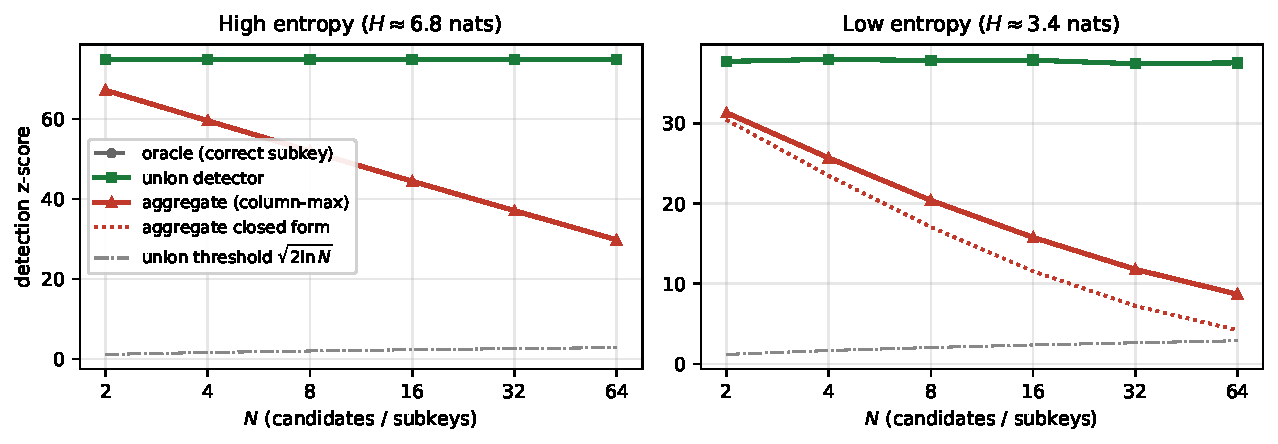
\includegraphics[width=0.98\linewidth]{figures/detector_comparison.pdf}
\end{center}
\caption{Union detection under $N$ subkeys
(simulation: $V{=}10^3$, $T{=}200$ tokens, $800$ runs). The union detector
coincides with the correct-subkey oracle at every $N$ and entropy level; its
only cost is the $\sqrt{2\ln N}$ threshold (dash-dotted, bottom).}
\label{fig:detectors}
\end{figure}

Two loss channels must not be conflated. The multiplicity cost above is the
\emph{only} price of restoring independence, and it is order-optimal:
detecting one elevated stream among $N$ independent nulls is the classical
needle-in-a-haystack problem, for which no index-blind level-$\alpha$ test can
improve on the max test's $\sqrt{2\ln N}$ threshold order
\citep{ingster1997,donoho2004higher}. Separately, \emph{reward selection
itself} tilts the released text toward weakly watermarked candidates --- a
loss that exists for any token-level watermark under any key design:

\begin{proposition}[Selection tilt]\label{prop:tilt}
If each candidate's (reward, per-text signal) pair is bivariate Gaussian with
correlation $\rho_{rs}$, i.i.d.\ across candidates, then hard-BoN selection
shifts the released signal by
$\mathbb E[z_{i^\ast}]-\mu_z=\rho_{rs}\,\sigma_z\,m_N$. With $\rho_{rs}<0$
(measured $\approx-0.5$) the post-selection signal declines at the
$\sqrt{2\ln N}$ rate --- the shape of Figure~\ref{fig:realshift} (right).
Proof in Appendix~\ref{app:proofs}.
\end{proposition}

\subsection{Instantiations}\label{sec:instantiations}
The framework specializes with no per-scheme work.
\emph{Gumbel/Aaronson} (our flagship, \S\ref{sec:experiments}): candidate $i$
runs strict argmax decoding with noise seeded by
$(\mathrm{SubKey}_i,\mathrm{ctx})$; the union wrapper reuses the standard
$\Gamma$-null detector.
\emph{Exponential / permute-and-flip samplers} \citep{zhao2024permute}: identical
treatment --- the noise is the same exponential family, so the detector carries
over verbatim.
\emph{Inverse-transform / random-offset schemes} \citep{kuditipudi2023robust}:
the lift replaces the random offset's approximate decorrelation with exact
(computational) independence while keeping their alignment detector per subkey.
\emph{Biased-logit schemes} (KGW): Theorem~\ref{thm:lifting}(a) applies ---
candidates become i.i.d.\ over the biased marginal, restoring ordinary BoN
behavior; closure in the sense of (b) is vacuous since the base scheme is not
distortion-free.

\section{Experiments}\label{sec:experiments}
\textbf{Setup.} We instantiate $\mathrm{JC}_N$ on the deployed Gumbel/Aaronson
scheme. LLaMA-3.1-8B-Instruct, HH-RLHF prompts ($128$), $N{=}16$
candidates, temperature $1.0$, ArmoRM reward; Gumbel/Aaronson watermark
(context hash $h{=}4$). Arms: unwatermarked i.i.d.\ BoN (ceiling); strict
shared-key; strict subkey (ours) with union detection; the softened shared-key
workaround of \citet{verma2025watermarking}. We report reward of the selected
output under four selection heads (single, hard-BoN, soft-BoN, Exp-BoN), detection
median $z$ and TPR, and calibration.

\begin{table}[t]
\caption{Main result (LLaMA-3.1-8B-Instruct, $N{=}16$). Strict shared key forfeits
the entire BoN gain; subkeys restore the unwatermarked ceiling at strict
distortion-freeness; union detection costs $\approx0.3$ z. The softened workaround
is dominated on all three axes.}
\label{tab:main}
\begin{center}
\begin{tabular}{llccc}
\toprule
Arm & Strategy & Reward & Median $z$ & TPR@$.01$ \\
\midrule
Unwatermarked (ceiling) & single & $0.0703$ & --- & --- \\
 & hard-BoN & $0.0848$ & --- & --- \\
\midrule
Softened shared key & single & $0.0697$ & $7.09$ & $0.944$ \\
\citep{verma2025watermarking} & hard-BoN & $0.0852$ & $5.62$ & $0.909$ \\
\midrule
Strict shared key & single & $0.0693$ & $8.00$ & $0.945$ \\
 & hard/soft/Exp-BoN & $0.0693$ & $8.00$ & $0.945$ \\
\midrule
\textbf{Strict subkey + union (ours)} & single & $0.0698$ & $7.71$ & $0.926$ \\
 & hard-BoN & $\mathbf{0.0861}$ & $6.50$ & $0.891$ \\
 & soft-BoN & $0.0746$ & $7.13$ & $0.915$ \\
 & Exp-BoN & $0.0750$ & $7.11$ & $0.911$ \\
\bottomrule
\end{tabular}
\end{center}
\end{table}

\textbf{Findings.}
(1) \emph{Collapse:} strict shared key yields $1.0/16$ unique candidates; all
selection heads return the single-sample reward $0.0693$ --- the full BoN gain
($+0.0155$) is forfeit.
(2) \emph{Restoration:} subkeys yield $16/16$ unique candidates; single-sample
reward $0.0698\approx0.0703$ (strict distortion-freeness), hard-BoN
$0.0861\ge0.0848$ (full gain; the slight excess is the watermark's variance bonus).
(3) \emph{Detection:} union costs $8.00\to7.71$ ($\approx0.3$ z); the subkey text is
null under the base key ($0.057$ at the $0.05$ level) and the union FPR is
calibrated ($0.055$/$0.012$ at $0.05$/$0.01$).
(4) \emph{Dominance:} vs.\ the softened workaround, ours is equal or better on
reward ($0.0861$ vs.\ $0.0852$), stronger on post-BoN detection ($z$ $6.50$ vs.\
$5.62$; strict argmax embeds a stronger per-text signal and union loses almost
nothing), and strictly distortion-free where softening is not.

\textbf{Selection shift vs.\ $N$ (real model).}
Figure~\ref{fig:realshift} is the real-data companion of Figure~\ref{fig:toy}:
subsampling $N\in\{1,\dots,16\}$ candidates and selecting by reward, the strict
shared key's gap to unwatermarked BoN grows from $0.0010$ to $0.0155$ ---
selection converts the joint degeneracy into a first-order, $N$-increasing bias
of the released output --- while the subkey arm stays at zero (slightly negative:
the variance bonus). The right panel tracks the watermark after selection: the
subkey arm's union $z$ exceeds the softened baseline at \emph{every} $N$.

\textbf{Selector family.}
Appendix~\ref{app:selectors} extends the evaluation to seven key-free
selectors from alignment practice (including rejection sampling and
diversity-preserving filter+sample) and two
key-dependent stress selectors: closure holds within noise for every key-free
selector, the theorem's key-independence side condition is empirically visible,
and a worst-case key-oracle evader still faces $0.938$ TPR.

\textbf{Second scheme family (permute-and-flip).}
Repeating the experiment with the permute-and-flip / exponential watermark
\citep{zhao2024permute} --- a different deterministic decoder with its own
detector --- reproduces both the failure and the fix
(Table~\ref{tab:pf}): the shared key again collapses to $1.0/16$ unique
candidates and forfeits the BoN gain ($0.0728$ vs.\ ceiling $0.0848$), and the
lifted version restores $16/16$ unique candidates and full BoN reward
($0.0874$; permute-and-flip's slightly sharper decoder even exceeds the
sampling ceiling, consistent with \citealp{zhao2024permute}). Union detection
calibrates exactly as in the Gumbel case (FPR $0.055/0.011$ at nominal
$0.05/0.01$; lifted text is null under the base key, $0.054$). One honest
difference: after reward selection the retained signal is weaker than for
Gumbel (median $z$ $4.27$, TPR $0.830$ at FPR $0.01$) --- the
reward--watermark anticorrelation is more pronounced for this scheme.

\textbf{Candidate diversity.}
Within-prompt statistics confirm closure at the sample level: the subkey arm is
statistically indistinguishable from unwatermarked sampling
(unique fraction $1.00$ vs.\ $1.00$, $3$-gram Jaccard $0.038$ vs.\ $0.039$,
shared word-prefix $1.10$ vs.\ $1.09$), the strict shared key is degenerate
(unique $0.06$, Jaccard $1.00$, shared prefix $154$ words --- the entire
generation), and the softened workaround retains a residual $2.2\times$ prefix
correlation ($2.45$ vs.\ $1.09$ words): softening decorrelates incompletely
\emph{and} sacrifices strict distortion-freeness.

\begin{figure}[t]
\begin{center}
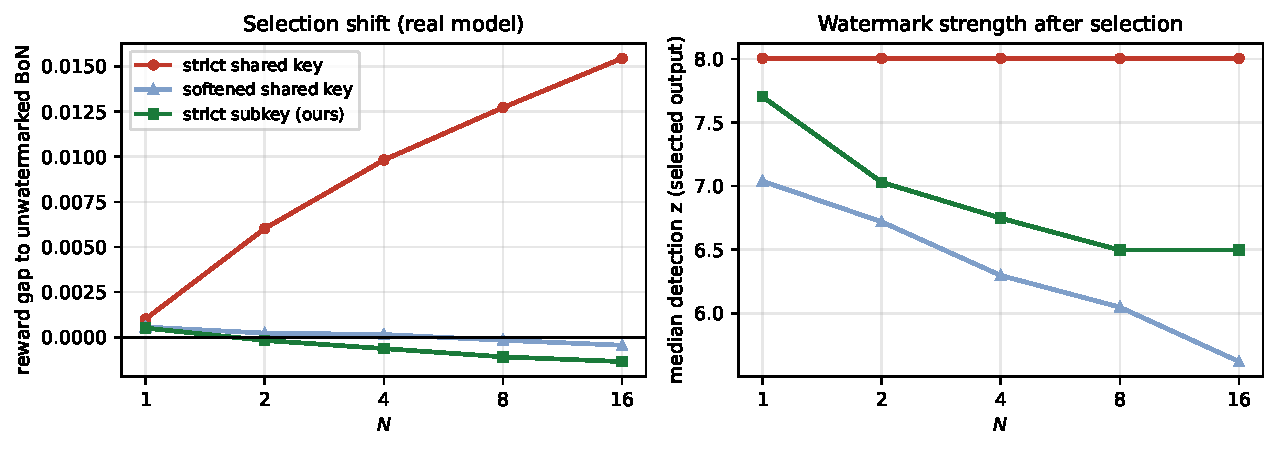
\includegraphics[width=0.98\linewidth]{figures/real_shift_vs_N.pdf}
\end{center}
\caption{Real-model selection shift (LLaMA-3.1-8B-Instruct, hard-BoN over
subsampled candidates). \emph{Left:} reward gap of the selected output to
unwatermarked BoN at the same $N$. The strict shared key's shift grows with $N$
(to $0.0155$, the entire BoN gain), mirroring Figure~\ref{fig:toy}; subkeys track
the ceiling (gap $\le 0$). \emph{Right:} median detection $z$ of the selected
output; the subkey arm (union detection) stays above the softened workaround at
every $N$. The shared key's flat $z=8.0$ reflects that its ``selection'' returns
the same single sample.}
\label{fig:realshift}
\end{figure}

% TODO: full detection-metric suite table (TPR/FPR/AUROC/F1/ANLPPT) + PPL — appendix B.
% TODO: second model pair for generality.

\section{Discussion}\label{sec:discussion}
\textbf{Security.} Multiple keys trade off against stealing/removal attacks
\citep{jovanovic2024stealing, nofreelunch2024}: more keys hide patterns better but
ease distribution estimation. Our setting is mild --- $N$ is small (2--16), the
subkeys are per-\emph{candidate} while only one candidate is released per query,
diluting an attacker's per-subkey sample budget by $N$ --- but the standard
trade-offs apply and deserve study.
\textbf{Scope.} Subkeys restore \emph{distributional} correctness; they do not
change the reward--watermark anticorrelation of the text itself (selection still
prefers weakly watermarked candidates; $z$ retained $79$--$95\%$ across heads),
which is an orthogonal, entropy-driven phenomenon. Intra-sequence key reuse
\citep{keycollision2024} is likewise orthogonal and composable with our fix.

\section{Conclusion}
Distortion-freeness, as certified, is a single-sample property; deployment is a
selection property. The gap is real (the entire BoN gain), the formalization is
simple ($N$-selection-closedness), and the remedy is not another watermarking
algorithm but a general compiler: $\mathrm{JC}_N$ lifts any keyed scheme ---
existing detectors included --- to selection-closedness under one master key,
at a once-per-sequence $\sqrt{2\ln N}$ detection cost. Watermarks should be
certified --- and can now be mechanically lifted --- to be distortion-free
\emph{after} you select.

\bibliography{refs}
\bibliographystyle{iclr2025_conference}

\appendix
\section{Proofs}\label{app:proofs}

\subsection{Notation and setting}
Fix a prompt $x$. Let $Q_x$ denote the unwatermarked single-sample law over
completions and $Q_x^{\otimes N}$ the law of $N$ i.i.d.\ samples. A watermarked
sampler with key $k\sim\mathcal K$ produces a candidate tuple
$\mathbf Y=(Y_1,\dots,Y_N)$ with joint law $P_x^{N}$ (all statements about $P$
are averaged over the key unless stated otherwise). A \emph{selection operator}
is a measurable map $S:\mathcal Y^{N}\times\mathcal U\to[N]$, where $U\sim\mu$ is
auxiliary randomness (e.g., a reward model's scores and tie-breaking)
independent of the watermark key; the released output is $Y_S$.

\subsection{Proof of Theorem~\ref{thm:closure}}
\textbf{Sufficiency (exact form).}
The map $\Phi:(\mathbf y,u)\mapsto y_{S(\mathbf y,u)}$ is measurable, and the law
of the released output is the pushforward $\Phi_\#(P_x^{N}\otimes\mu)$. If
$P_x^{N}=Q_x^{\otimes N}$ then
$\Phi_\#(P_x^{N}\otimes\mu)=\Phi_\#(Q_x^{\otimes N}\otimes\mu)$, which is exactly
the law of unwatermarked Best-of-$N$ under the same selector. Since $\Phi$ was
arbitrary, closure holds for \emph{every} selector simultaneously.

\textbf{Sufficiency (computational form).}
Suppose $P_x^{N}$ and $Q_x^{\otimes N}$ are computationally indistinguishable and
$S$ runs in polynomial time. Any polynomial-time distinguisher $D$ acting on the
released output induces the distinguisher $D\circ\Phi$ acting on the candidate
tuple (sampling $U$ internally), with identical advantage. Hence the released
outputs are indistinguishable.

\textbf{Necessity (probe selectors).}
Assume (ii). Constant selectors $S\equiv i$ force every marginal to equal
$Q_x$. We show by induction on $k$ that every $k$-dimensional joint
factorizes. For $k=2$ and $i\ne j$, use the probe ``$S=i$ if $Y_j\in B$, else
$j$'': its output law on $A$ is
$P(Y_i\in A,Y_j\in B)+P(Y_j\in A,Y_j\notin B)$; the second term equals
$Q_x(A\cap B^c)$ by the marginal step, and the i.i.d.\ reference value is
$Q_x(A)Q_x(B)+Q_x(A\cap B^c)$, so $P(Y_i\in A,Y_j\in B)=Q_x(A)Q_x(B)$.
For the step $k{-}1\to k$, fix distinct coordinates $i,t_1,\dots,t_{k-1}$ and
sets $A,B_1,\dots,B_{k-1}$; write $E=\bigcap_m\{Y_{t_m}\in B_m\}$, pick
$j=t_1$, and use the probe ``$S=i$ if $E$, else $j$''. Its output law on $A$
is $P(Y_i\in A,E)+P(Y_j\in A,E^c)$; the second term is
$P(Y_j\in A)-P(Y_j\in A,E)$, and $P(Y_j\in A,E)$ merges the two occurrences
of $Y_j$ into $\{Y_j\in A\cap B_1\}$, hence is a $(k{-}1)$-dimensional joint,
which factorizes by induction and matches the i.i.d.\ reference. Subtracting
yields $P(Y_i\in A,E)=Q_x(A)\prod_m Q_x(B_m)$. Cylinder sets generate the
product $\sigma$-algebra, so the joint equals $Q_x^{\otimes N}$. The
computational version follows by quantitative bookkeeping of the same probes.
\qed

\textbf{Insufficiency of marginal preservation.}
The following minimal example shows that exact marginals give no control
whatsoever over the selected output; it is the formal core of
Figure~\ref{fig:toy} and of the real-model collapse in
Table~\ref{tab:main}.

\begin{example}[Comonotone candidates]\label{ex:comonotone}
Let the outcome space be $\{0,1\}$ with $Q_x(\{1\})=\tfrac12$, and let the reward
satisfy $r(1)>r(0)$ so that the selector returns $1$ whenever some candidate
equals $1$. Consider the comonotone coupling $Y_1=\dots=Y_N$ with
$Y_1\sim Q_x$ --- every marginal is exact. Unwatermarked Best-of-$N$ releases $1$
with probability $1-2^{-N}$; the comonotone sampler releases $1$ with probability
$\tfrac12$. The total-variation shift of the released output is therefore
\[
\mathrm{TV}=\tfrac12-2^{-N}\;\xrightarrow{N\to\infty}\;\tfrac12 ,
\]
monotonically increasing in $N$. The shared-key deterministic scheme of
\S\ref{sec:collapse} realizes exactly this coupling (all candidates identical),
so the bound is attained by a deployed system, not only in the worst case. \qed
\end{example}

\subsection{Proof of Proposition~\ref{prop:hierarchy}}
\textbf{(i) $N$-selection-closedness $\Rightarrow$ marginal
distortion-freeness.} Take the selector $S\equiv 1$ (release the first
candidate); closure for this selector is precisely marginal preservation.

\textbf{(ii) Marginal $\not\Rightarrow$ closed.} Example~\ref{ex:comonotone}: the
comonotone sampler is marginally exact and fails $2$-selection-closedness with
$\mathrm{TV}=\tfrac14$.

\textbf{(iii) Undetectability $\Rightarrow$ closure (computational).} An
adversary in the undetectability game of \citet{christ2023undetectable} may issue
the same prompt $N$ times, obtaining (by the multi-query guarantee) a tuple
computationally indistinguishable from $N$ unwatermarked calls. A
polynomial-time distinguisher between $P_x^{N}$ and $Q_x^{\otimes N}$ is thus
literally a distinguisher in the undetectability game, so undetectability
implies indistinguishability of the joints; conclude with
Theorem~\ref{thm:closure}.

\textbf{(iv) Closed $\not\Rightarrow$ undetectable.} The subkey construction with
strict (argmax) decoding is $N$-selection-closed by construction, yet it is not
undetectable: for a fixed candidate index the map from context to token is
deterministic, so an observer issuing many queries with a shared prefix sees
response collisions at a rate far exceeding that of genuine sampling --- a
polynomial-time, key-free distinguisher. (This is a property of the entire
context-hash family, orthogonal to our fix.) Hence the inclusion is strict.
\qed

\subsection{Proof of Theorem~\ref{thm:lifting}}
\textbf{(a) Ideal tier.} With truly independent streams the candidates are
independent runs of the unmodified base sampler by construction, hence i.i.d.\
with law $\mu_W$; the joint \emph{equals} $\mu_W^{\otimes N}$ and every
pushforward is preserved exactly.
\textbf{(b) Real tier.} All subkeys are evaluations of one PRF at distinct points
$(\mathrm{MasterKey},i)$, $i\in[N]$; by PRF security the tuple of derived noise
streams is computationally indistinguishable from $N$ independent truly-random
streams (a single invocation of the PRF game over the $N$ query points; no
hybrid over candidates is needed). Conditioned on independent streams, the
candidates are independent runs of the unmodified base sampler $W$, hence
i.i.d.\ with law $\mu_W$; a distinguisher against the candidate tuple would
therefore distinguish the streams, contradicting PRF security. Note that
(a)--(b) make no assumption on $W$ beyond keyed-ness --- in particular no
distortion-freeness.
\textbf{(c)} If $\mu_W=Q_x$ for every prompt, then i.i.d.\ with marginal $Q_x$
is precisely Definition~\ref{def:closure}, and Theorem~\ref{thm:closure} yields
closure under every selection operator.
\textbf{(d)} The base detector's null is exact under each wrong subkey (the
text is independent of that subkey's stream), so the union wrapper of
Proposition~\ref{prop:union} applies verbatim, with its once-per-sequence
multiplicity cost and index-recovery byproduct. \qed

\subsection{Proofs of Lemma~\ref{lem:attenuation} and Proposition~\ref{prop:tilt}}
\emph{Lemma~\ref{lem:attenuation}.} Write the equicorrelated vector as
$X_i=\mu+\sigma(\sqrt{\rho}\,Z_0+\sqrt{1-\rho}\,Z_i)$ with independent
standard normals $Z_0,Z_1,\dots,Z_N$. Then
$\max_i X_i=\mu+\sigma\sqrt{\rho}\,Z_0+\sigma\sqrt{1-\rho}\,\max_i Z_i$, and
taking expectations kills the shared factor:
$\mathbb E[\max_i X_i]=\mu+\sigma\sqrt{1-\rho}\,m_N$. \qed

\emph{Proposition~\ref{prop:tilt}.} Regress the signal on the reward:
$z_i=\mu_z+\rho_{rs}\sigma_z(R_i-\mu_R)/\sigma_R+\eta_i$ with $\eta_i$
independent of the rewards. Selecting $i^\ast=\arg\max_i R_i$ and taking
expectations, $\mathbb E[\eta_{i^\ast}]=0$ (the selection is measurable in the
rewards alone), so
$\mathbb E[z_{i^\ast}]=\mu_z+\rho_{rs}\sigma_z\,
\mathbb E[R_{i^\ast}-\mu_R]/\sigma_R=\mu_z+\rho_{rs}\sigma_z m_N$ for
i.i.d.\ Gaussian rewards. \qed

\subsection{Detection under $N$ subkeys}\label{app:detection}
We work in the location-shift signal model of \S\ref{sec:detection}: token
scores under the correct subkey at watermarked positions are i.i.d.\
$\mathrm{Gumbel}(\Delta,1)$; under any incorrect subkey, and at any position of
unwatermarked text, scores are i.i.d.\ $\mathrm{Gumbel}(0,1)$, independent
across subkeys --- independence holds because distinct subkeys read disjoint
PRF domains (exactly in the ideal tier, computationally in the real tier);
this is what licenses \emph{exact} null calibration (\v{S}id\'ak or
empirical quantiles) in place of the conservative Bonferroni bound, cf.\ the
matched-FPR evaluation of Appendix~\ref{app:exp}. For uniform logits over a nucleus of size $V$ the model is exact
with $\Delta=\ln V$ (the winning token's noise is the maximum of $V$ i.i.d.\
Gumbels, i.e., $\mathrm{Gumbel}(\ln V,1)$); for peaked distributions it is an approximation.
Throughout, $\gamma$ is Euler's constant,
$\sigma_g^2=\pi^2/6$, and $T$ is the number of scored tokens.

\begin{proposition}[Union detector]\label{prop:union}
For each subkey $i$ let
$z_i=\big(\sum_{t\le T} g_i(x_t)-T\gamma\big)/(\sigma_g\sqrt T)$ and let the
union detector reject when $\max_i z_i$ exceeds the $(1-\alpha/N)$-quantile of
the single-key null. Then:
(a) the false-positive rate is at most $\alpha$ for \emph{any} dependence among
the $z_i$ (Bonferroni), and the null quantile inflation is
$\sqrt{2\ln N}\,(1+o(1))$ in z-units;
(b) under the signal model, the correct subkey satisfies
$\mathbb E[z_{i^*}]=\sqrt T\,\Delta/\sigma_g$, so the power of the union test
equals that of the oracle test up to the additive threshold term:
the z-margin is $\sqrt T\,\Delta/\sigma_g-\sqrt{2\ln N}-z_\alpha$, and the
relative loss vanishes as $T\to\infty$;
(c) $\arg\max_i z_i$ recovers the selected candidate's index with probability
$\to1$ in the same limit.
\end{proposition}
\begin{proof}
(a) is the union bound; the quantile of the maximum of $N$ standard (Gumbel-sum,
asymptotically normal) nulls grows as $\sqrt{2\ln N}$.
(b) Linearity of expectation for the correct subkey; the incorrect subkeys'
maximum is $O_P(\sqrt{2\ln N})$, so for
$\sqrt T\,\Delta/\sigma_g>\sqrt{2\ln N}$ the maximum is attained by the correct
subkey with probability $\to1$, which also gives (c).
\end{proof}

\section{Experimental Details}\label{app:exp}

\subsection{Configuration}
Generator: LLaMA-3.1-8B-Instruct (fp16, single A100-40GB per arm); prompts: $128$
from Anthropic HH-RLHF (test split), raw format; $N{=}16$ candidates per prompt,
nucleus sampling $p{=}0.95$, temperature $1.0$, generation length $200$ tokens.
Watermark: Gumbel/Aaronson with context hash over the preceding $h{=}4$ tokens
(hash chain $s\!\leftarrow\!(s\cdot\texttt{salt}+\mathrm{token})\bmod(2^{64}{-}1)$,
master seed $42$); the subkey arm appends a domain-separation step
$s\!\leftarrow\!(s\cdot\texttt{salt}+c_0+i)\bmod(2^{64}{-}1)$ with candidate index
$i$. Reward: ArmoRM-Llama3-8B-v0.1. Detection: per-key score
$\sum_t\log\frac{1}{1-r_{x_t}}$ with exact $\Gamma(n,1)$ null; union arm reports
$\min(1,N\cdot\min_i p_i)$. Selection heads: hard-BoN ($\arg\max$ reward),
soft-/Exp-BoN ($\arg\max$ of $r/\lambda$ plus Gumbel/exponential noise,
$\lambda{=}0.02$). BoN at $N<16$ uses repeated subsampling of the $16$ generated
candidates ($60$--$80$ resamples per prompt). Wall-clock: generation
$\approx13.5$\,min per arm ($128\times16$ candidates, one GPU); union detection is
$N$ single-key passes (embarrassingly parallel), $\approx4.5$\,min for
$2048$ texts at $N{=}16$ on one GPU.

\subsection{Full metric suite}
Table~\ref{tab:suite} reports the complete detection suite for the selected
output (hard-BoN, $N{=}16$) and for single samples: median $z$, TPR at nominal
$p<0.05/0.01$, the matched detector's FPR on unwatermarked text, AUROC, F1 at
$p<0.05$, the length-normalized ANLPPT ($-\ln p$ per token), and median
perplexity under the generating model. Notes: (i) at \emph{nominal} thresholds
the two detectors are miscalibrated in opposite directions --- the union's
Bonferroni correction is conservative (realized FPR $0.039/0.008$ at nominal
$0.05/0.01$) while the softened baseline's analytic null is anti-conservative
on real text (realized FPR $0.062/0.016$, i.e.\ $1.6\times$ nominal) --- so
nominal-threshold TPRs are not comparable across arms.
(ii) The strict decoder embeds a visibly stronger per-token signal than the
softened sampler (single-sample ANLPPT $0.255$ vs.\ $0.201$), which survives
selection ($0.154$ vs.\ $0.137$). (iii) Perplexity is preserved throughout
(subkey $3.9/3.5$ vs.\ unwatermarked $3.8/3.3$, single/BoN).

\paragraph{Matched-FPR comparison (exact empirical calibration).}
The fair comparison sets each detector's threshold at the empirical quantile of
its \emph{own} null (unwatermarked text under the same detector), so both arms
are evaluated at identical realized FPR. Since the $N$ subkey scores on a given
text are independent, the union null is exactly calibratable; empirical
calibration additionally absorbs the finite-text slack of the analytic
$\Gamma$-null. For the selected output (hard-BoN, $N{=}16$):

\begin{center}
\small
\begin{tabular}{lccc}
\toprule
Arm (selected output) & TPR@FPR$=.05$ & TPR@FPR$=.01$ & TPR@FPR$=.001$ \\
\midrule
Softened shared key & $\mathbf{0.948}$ & $0.882$ & $0.866$ \\
Strict subkey $+$ union (ours) & $0.930$ & $\mathbf{0.891}$ & $\mathbf{0.883}$ \\
\bottomrule
\end{tabular}
\end{center}

Under honest calibration the softened baseline's apparent nominal-threshold
advantage disappears: its TPR@$.01$ drops from $0.909$ to $0.882$ (its nominal
threshold had operated at FPR $0.016$), while ours is unchanged
($0.891$). At the strict operating points that matter for deployment
(FPR $10^{-2}$, $10^{-3}$) the subkey arm leads, and its ROC degrades more
gracefully as the threshold tightens ($0.930\!\to\!0.883$ vs.\
$0.948\!\to\!0.866$) --- the payoff of the stronger median signal
($z$ $6.50$ vs.\ $5.62$). At the loose $0.05$ point the softened arm retains a
small edge from the union's heavier max-of-$N$ null tail.

\begin{table}[h]
\caption{Full metric suite (LLaMA-3.1-8B-Instruct; selected $=$ hard-BoN
$N{=}16$; thresholds at nominal $p$). PPL is median perplexity under the
generating model; unwatermarked reference PPL is $3.8$ (single) / $3.3$ (BoN).}
\label{tab:suite}
\begin{center}
\small
\setlength{\tabcolsep}{4pt}
\begin{tabular}{llccccccccc}
\toprule
Arm & Mode & Reward & Med.\ $z$ & TPR$_{.05}$ & TPR$_{.01}$ & FPR$_{.05}$ & FPR$_{.01}$ & AUROC & ANLPPT & PPL \\
\midrule
Softened & single & $0.0697$ & $7.09$ & $0.969$ & $0.944$ & $0.061$ & $0.016$ & $0.992$ & $0.201$ & $4.2$ \\
         & selected & $0.0852$ & $5.62$ & $0.956$ & $0.909$ & $0.062$ & $0.016$ & $0.986$ & $0.137$ & $3.7$ \\
\midrule
Strict shared & single & $0.0693$ & $8.00$ & $0.953$ & $0.945$ & $0.061$ & $0.016$ & $0.986$ & $0.255$ & $3.7$ \\
              & selected & $0.0693$ & $8.00$ & $0.953$ & $0.945$ & $0.062$ & $0.016$ & $0.986$ & $0.255$ & $3.7$ \\
\midrule
Strict subkey & single & $0.0698$ & $7.71$ & $0.948$ & $0.926$ & $0.062$ & $0.013$ & $0.982$ & $0.222$ & $3.9$ \\
(union) & selected & $0.0861$ & $6.50$ & $0.930$ & $0.891$ & $0.039$ & $0.008$ & $0.973$ & $0.154$ & $3.5$ \\
\bottomrule
\end{tabular}
\end{center}
\end{table}

\subsection{Candidate diversity}
Within-prompt statistics over the $16$ candidates (pairwise over the first $8$):

\begin{center}
\small
\begin{tabular}{lccc}
\toprule
Arm & Unique fraction & $3$-gram Jaccard & Shared word-prefix \\
\midrule
Unwatermarked & $1.00$ & $0.039$ & $1.09$ \\
Strict subkey (ours) & $1.00$ & $0.038$ & $1.10$ \\
Softened shared key & $1.00$ & $0.037$ & $2.45$ \\
Strict shared key & $0.06$ & $1.000$ & $154.3$ \\
\bottomrule
\end{tabular}
\end{center}

The subkey arm matches unwatermarked sampling on all three statistics; the
softened workaround retains a $2.2\times$ residual prefix correlation (candidates
start identically until the multinomial happens to diverge, then decorrelate);
the strict shared key shares the entire generation.

\subsection{Selector family}\label{app:selectors}
Theorem~\ref{thm:closure} promises closure for \emph{every} selection operator
that is independent of the watermark key. We test seven key-free selectors
drawn from alignment practice --- single, uniform-random (control),
hard-/soft-/Exp-BoN, rejection sampling (accept the first candidate with reward
above the unwatermarked median, random scan order), and filter+sample (discard
the bottom half by reward, sample uniformly among survivors --- the standard
diversity-preserving softening) --- and two \emph{key-dependent} stress selectors
that deliberately violate the theorem's side condition: adversarial min-$z$
(an evader with a key oracle picks the weakest-watermarked candidate) and
max-$z$ (WaterMax-style watermark boosting). All at $N{=}16$.

\begin{table}[h]
\caption{Selector family. Left: closure check --- reward gap of each arm to
unwatermarked BoN under the \emph{same} selector (per-prompt SE
$\approx0.0024$). Right: watermark after selection for the subkey arm.
Key-free selectors: subkey gaps are within noise across all seven, while the
strict shared key loses under every selector; the key-dependent selectors sit
outside the theorem's scope and visibly break the match --- an empirical
demarcation of the side condition.}
\label{tab:selectors}
\begin{center}
\small
\setlength{\tabcolsep}{4.5pt}
\begin{tabular}{llrrr|cc}
\toprule
 & & \multicolumn{3}{c|}{Reward gap to unwm} &
 \multicolumn{2}{c}{Subkey watermark} \\
Selector & Key-free & shared & softened & subkey & med.\ $z$ & TPR@FPR$_{.01}$ \\
\midrule
single        & yes & $-0.0010$ & $-0.0006$ & $-0.0006$ & $7.71$ & $0.917$ \\
random        & yes & $-0.0006$ & $-0.0009$ & $-0.0001$ & $7.95$ & $0.914$ \\
hard-BoN      & yes & $-0.0154$ & $+0.0004$ & $+0.0013$ & $6.47$ & $0.891$ \\
soft-BoN      & yes & $-0.0047$ & $-0.0000$ & $+0.0006$ & $7.24$ & $0.992$ \\
Exp-BoN       & yes & $-0.0049$ & $-0.0001$ & $+0.0007$ & $7.05$ & $0.992$ \\
rejection     & yes & $-0.0058$ & $-0.0003$ & $+0.0018$ & $6.85$ & $0.922$ \\
filter+sample & yes & $-0.0075$ & $-0.0002$ & $+0.0004$ & $6.88$ & $0.977$ \\
\midrule
\multicolumn{7}{l}{\emph{Stress tests (non-deployment; violate the key-independence side condition):}} \\
adv.\ min-$z$ & \textbf{no} & $-0.0014$ & $+0.0043$ & $+0.0053$ & $3.98$ & $0.938$ \\
max-$z$       & \textbf{no} & $+0.0000$ & $-0.0101$ & $-0.0113$ & $13.15$ & $0.984$ \\
\bottomrule
\end{tabular}
\end{center}
\end{table}

Observations. (i) \emph{Closure is selector-universal}: the subkey arm matches
unwatermarked BoN within noise under all seven key-free selectors, while the
strict shared key loses under every one of them (there is nothing to select
from). (ii) \emph{The theorem's side condition is visible in data}: the two
key-dependent selectors break the match ($+0.0053$/$-0.0113$), exactly as
predicted --- closure requires the selector to be independent of the key.
(iii) \emph{Evasion}: even a worst-case evader with a key oracle, picking the
weakest of $16$ candidates, only reduces the median $z$ from $7.7$ to $4.0$ and
is still detected at $0.938$ TPR at matched FPR $0.01$; the derandomized shared
key is evasion-immune ($z{=}8.0$ under every selector) but selection-dead ---
a clean statement of the diversity/evasion trade.
(iv) \emph{Watermark boosting} composes with the framework: max-$z$ selection
lifts the median $z$ to $13.2$ at a $0.011$ reward cost, a WaterMax-style
operating point. (v) \emph{Likelihood-rank gradient}: ordering the candidate set by sequence
likelihood reveals a monotone gradient --- reward falls from $0.073$ to
$0.059$ and median $z$ rises from $4.7$ to $12.9$ across ranks --- i.e.,
model-typical text is simultaneously reward-preferred and watermark-poor, the
within-set mirror of the reward--watermark anticorrelation (and the reason
reward selection mildly weakens any token-level watermark).

\subsection{Second scheme family: permute-and-flip}
\begin{table}[h]
\caption{The collapse and the lift on a second scheme family
(permute-and-flip; LLaMA-3.1-8B-Instruct, $N{=}16$, hard-BoN; TPR at matched
empirical FPR $0.01$). Same pattern as Gumbel: shared key collapses and
forfeits the BoN gain; the lift restores i.i.d.\ candidates and full reward at
a small union-detection cost.}
\label{tab:pf}
\begin{center}
\small
\begin{tabular}{llcccc}
\toprule
Arm & Mode & Unique/16 & Reward & Med.\ $z$ & TPR@$.01$ \\
\midrule
Unwatermarked (ceiling) & hard-BoN & $16$ & $0.0848$ & --- & --- \\
\midrule
PF strict shared key & single & \multirow{2}{*}{$1.0$} & $0.0728$ & $6.47$ & $0.922$ \\
 & hard-BoN & & $0.0728$ & $6.47$ & $0.938$ \\
\midrule
PF lifted (subkey $+$ union) & single & \multirow{2}{*}{$16.0$} & $0.0716$ & $6.02$ & $0.859$ \\
 & hard-BoN & & $\mathbf{0.0874}$ & $4.27$ & $0.830$ \\
\bottomrule
\end{tabular}
\end{center}
\end{table}
Notes: permute-and-flip is distortion-free with respect to its \emph{own}
decode law (not the sampling law), so the inherited joint guarantee is
``i.i.d.\ from the PF-decode law''; accordingly the shared-key and lifted
single-sample rewards agree within noise ($0.0728$ vs.\ $0.0716$), and the
lifted BoN slightly exceeds the \emph{sampling} ceiling because the PF decoder
is mildly sharper. Union calibration: FPR $0.055/0.011$ at nominal $0.05/0.01$;
lifted text under the base key is null ($0.054$ at the $0.05$ level).

\subsection{Calibration}
Union detector on unwatermarked text ($128$ prompts $\times16$ candidates):
realized FPR $0.055/0.012$ at nominal $0.05/0.01$ before Bonferroni tightening
of the selected-output evaluation ($0.039/0.008$, Table~\ref{tab:suite});
subkey-generated text scored under the \emph{base} key is null
($0.057$ at the $0.05$ level), confirming cryptographic separation of the
derived streams.

\end{document}
